\input{../header}
\usepackage{pgfplots}
\rhead{Your name: \rule{8cm}{0.15mm}}

\begin{document}

\section{Learning target DF1, version 1}

Estimate the value of a derivative using difference quotients, and draw corresponding secant and tangent lines on the graph of a function.

\hrulefill


\everymath{\displaystyle}

Suppose that you know the following values of some function $g(x)$:

\[
\begin{array}{c||r|r|r}
      x  &  1.7 &  2   &  2.3 \\\hline
    g(x) & -2.2 & -2   & -1.5
\end{array}
\]
\begin{enumerate}[leftmargin=0pt]

\item Plot these points and sketch a plausible graph of $g(x)$.

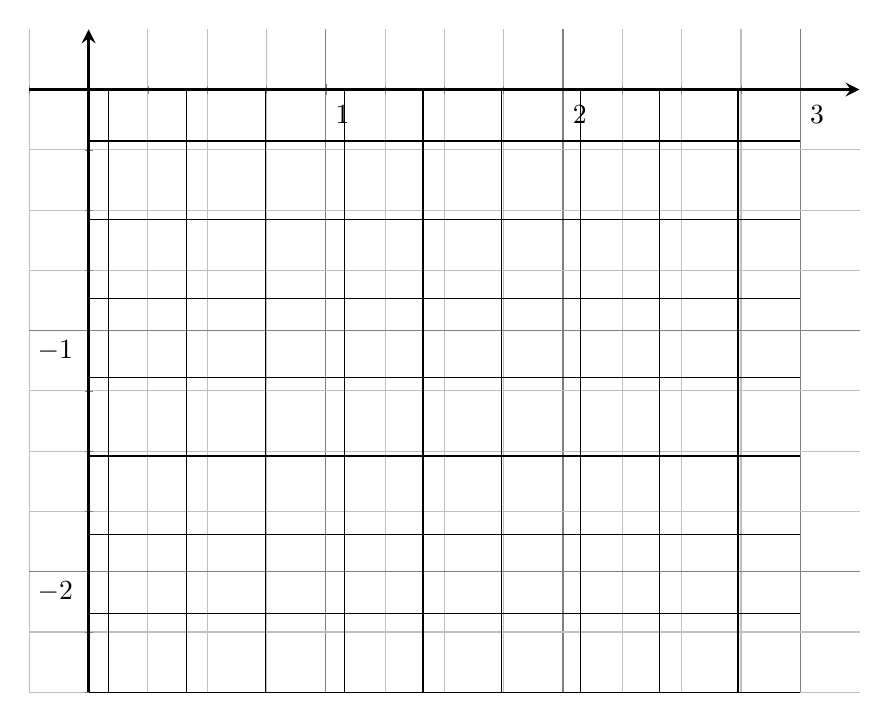
\begin{tikzpicture}
    \begin{axis}[
        width=\textwidth, height=10cm,
        xmin=-0.25, xmax=3.25, ymin=-2.5, ymax=0.25,
        xtick distance = 1, ytick distance = 1,
        minor tick num = 3,
        xticklabel style={anchor=north west},
        yticklabel style={anchor=north east},
        major grid style={thin, black!50},
        grid=both, 
        axis lines=center, axis line style = very thick]
        \draw (0,0) grid (3, -3);
    \end{axis}
\end{tikzpicture}

\item On your graph above, draw a plausible tangent line to the graph of $g(x)$ at $x=2$.

\item Use a central difference to estimate $g'(2)$. Draw the corresponding secant line on your graph above.

\vfill

\item Compute another, different estimate of $g'(2)$. Draw the corresponding secant line on your graph.

\vfill

\item Which one of your approximations is the best? How do you know?

\vspace{1cm}

\end{enumerate}

%%%%%%%%%%%%%%%%%%%%%%%%%%%%%%%%%%%%%%%%%%%%%%%%%%%%%%%%%
\pagebreak
%%%%%%%%%%%%%%%%%%%%%%%%%%%%%%%%%%%%%%%%%%%%%%%%%%%%%%%%%

\section{Learning targets DF1 and DFa, version 2}

Arapaho Glacier is a mountain glacier in Roosevelt National Forest,
west of Boulder, CO. The following table\footnote{
Haugen, B., Scambos, T., Pfeffer, T., \& Anderson, R. (2010). Twentieth-century changes in the thickness and extent of Arapaho Glacier, Front Range, Colorado. \textit{Arctic, Antarctic, and Alpine Research, 42}(2), 198-209.}
gives the surface area, $A(t)$, in square meters, of Arapaho Glacier in the year $t$. 
\begin{center}
	\begin{tabular}{|c|c|c|c|c|}
	\hline
	$t$ & 1900 & 1960 & 1973 & 1999\\
	\hline
	$A(t)$ & 338,282 & 250,764 & 225,000 & 162,027\\
	\hline
	\end{tabular}
 \end{center}
	
\begin{enumerate}[leftmargin=0pt]

\item Compute an approximation for $A'(1960)$, and {\bf include units} for this number.
\vfill
\item Write a sentence explaining what the number means about how the area of the glacier is changing.\\
\textbf{Don't say ``per,'' and don't say ``rate.''}

\vfill
\vfill

\item Compute an approximation for $A'(1999)$, and {\bf include units} for this number.\\
Do you think your approximation is too high or too low? Why?

\vfill
\vfill

\item How does $A'(1960)$ compare to $A'(1999)$? Is that good or bad?
\vfill
\end{enumerate}

%%%%%%%%%%%%%%%%%%%%%%%%%%%%%%%%%%%%%%%%%%%%%%%%%%%%%%%%%
\pagebreak
%%%%%%%%%%%%%%%%%%%%%%%%%%%%%%%%%%%%%%%%%%%%%%%%%%%%%%%%%

\section{Learning target DF1, version 3}


Estimate the value of a derivative using difference quotients, and draw corresponding secant and tangent lines on the graph of a function.

\hrulefill


Below is a graph of the function $\displaystyle f(x)=\frac{x^4}{12}-\frac{x^2}{2}-x$. 
\begin{center}
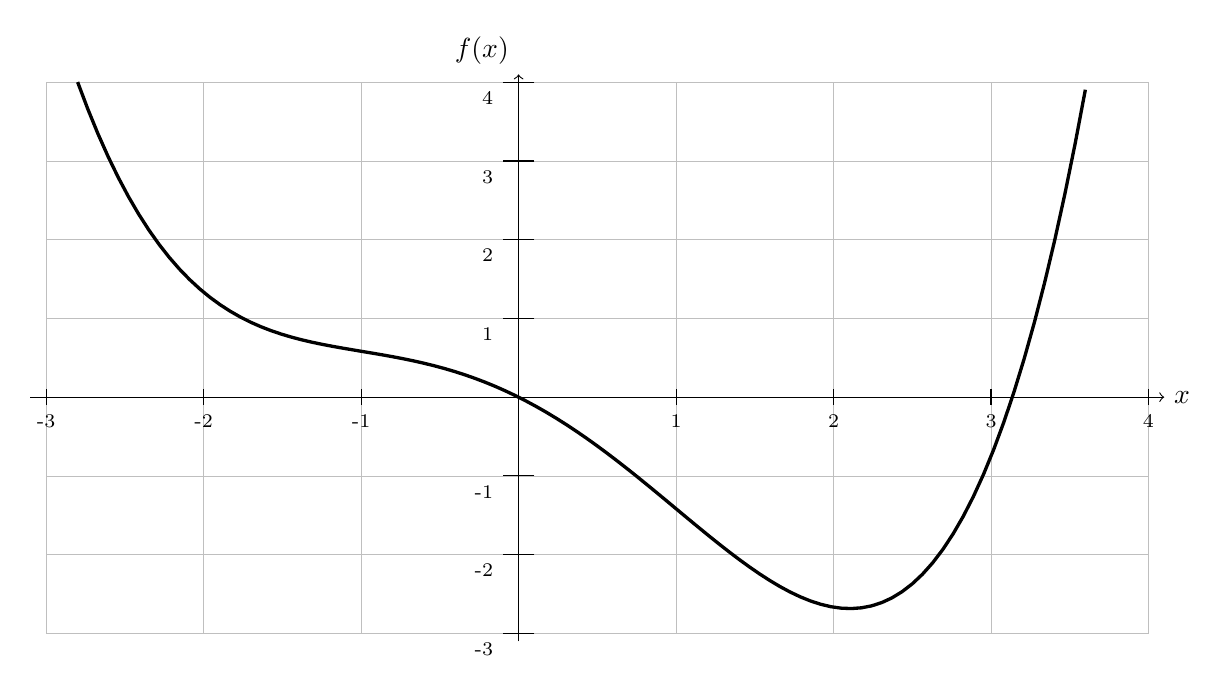
\begin{tikzpicture}[domain=-4:4, xscale = 2, yscale = 1] 
%grid and axis: 
\draw[very thin, color=lightgray] (-3,-3) grid (4,4);
\draw[->] (-3.1, 0) -- (4.1, 0) node[right] {$x$};
\draw[->] (0, -3.1) -- (0, 4.1) node[above left] {$f(x) $};

%x-axis labels:
\foreach \i in {-3,-2,-1,1, 2, 3,4} {
	\draw (\i, .1) -- (\i, -.1) node[below] {\scriptsize \i};
}
%y-axis labels:
\foreach \i in {-3,-2,-1, 1, 2, 3, 4} {
	\draw (.1,\i) -- (-.1, \i) node[below left] {\scriptsize \i};
}
\draw[very thick, color=black, domain=-2.8:3.6, samples=100] plot (\x,{0.08333*\x*\x*\x*\x-0.5*\x*\x-\x}) node[] {};
\end{tikzpicture}
\end{center}

\begin{enumerate}[(a)]
\item On the graph above, draw the tangent line to the curve at $x=-1$. 

\item On the graph above, draw a secant line that goes through the curve at $x=-1$ and at some other nearby $x$-value of your choice.

\item Calculate the slope of that secant line.

\vfill

\item Use $f'(x)$ to calculate the slope of the tangent line. Compare the value you get here to the value you got in part (c). Does that make sense?

\vfill
\end{enumerate}

%%%%%%%%%%%%%%%%%%%%%%%%%%%%%%%%%%%%%%%%%%%%%%%%%%%%%%%%%
\pagebreak
%%%%%%%%%%%%%%%%%%%%%%%%%%%%%%%%%%%%%%%%%%%%%%%%%%%%%%%%%


\section{Learning target DF1, version 4}

Estimate the value of a derivative using difference quotients, and draw corresponding secant and tangent lines on the graph of a function.

\hrulefill

A water balloon is tossed vertically in the air from a window. The balloon's height (measured in feet) at time $t$ (measured in seconds after being launched) is given by \(s(t) = -16t^2 + 16t + 32\); \\
a graph of this function is provided below.

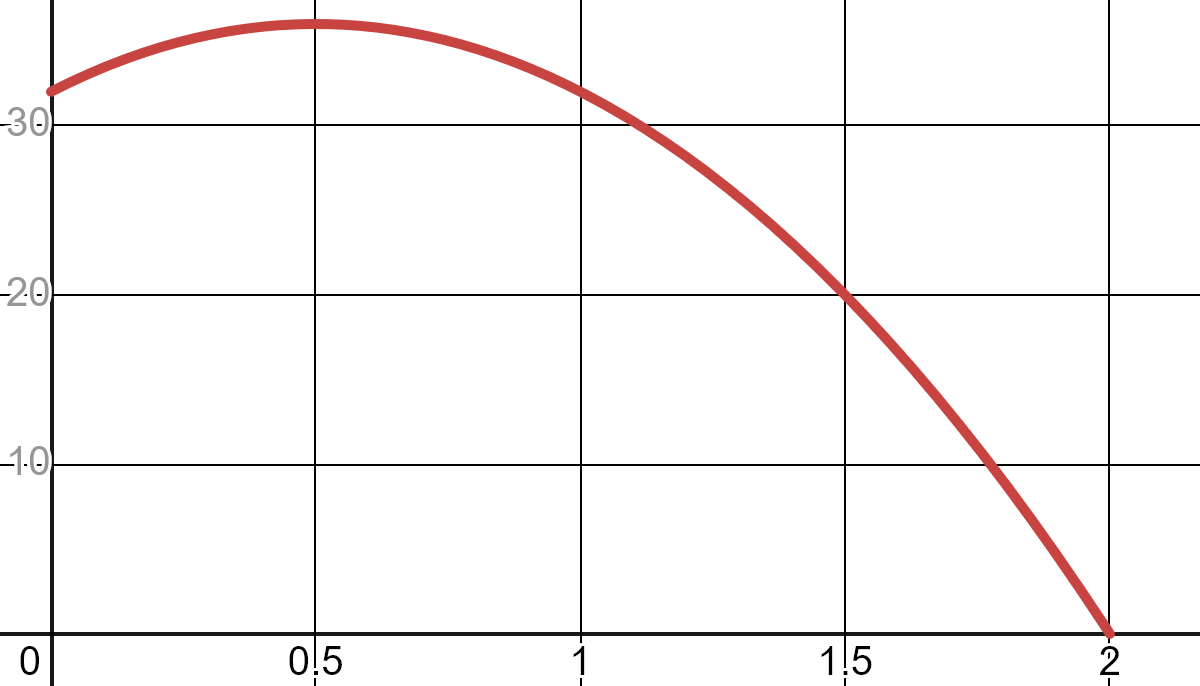
\includegraphics[width=\textwidth]{../images/DF1-v4.png}

\begin{enumerate}[(a)]
    \item Compute $s(1)$. Show your work.
    \vfill
    \item On the graph above, carefully sketch the \textit{tangent} line to $s(t)$ at $t=1$.
    \item On the graph above, carefully sketch a \textit{secant} line through the point on the graph at $t=1$ and a second nearby point.
    \item Compute the slope of your secant line. Show your work. 

    \vspace{-0.7em}
    {\tiny Hints: rise over run; one of your two $y$-values is $s(1)$, which you computed in part (a).}
    \vfill
    \item Use shortcut rules to find $s'(t)$, and compute $s'(1)$; show your work. Compare your result here to your result in part (d). Do these two numbers make sense together? Why?
    \vfill
\end{enumerate}

\end{document}